\chapter{Concept}
\label{ch:concept}

This chapter describes in detail the conceptual aspects of this thesis. The concept is divided into three phases, in the first phase data collection and cleaning will be described, in the next phase resampling of data and clustering will be described and in the last phase, description of machine learning models and the evaluation strategies will be described.

\section{Phase 1: Data Collection and Cleaning}
In the first phase, the data collection techniques are desribed in detail, also how and why the data was cleaned in order to make it suitable for machine learning algorithm is described. 

\subsection*{Data Collection}
Legal laws are written to be applicable in various situations. For example, a law for agricultural products may be applicable in situations where trading of goods happens.  High-level categories of multilingual legal documents provided by the European Union help to navigate in the legislative corpus,  they are also comprised of many languages so that can be used by various Nations. The applicability of these legal texts in various situations makes the classification of these texts on the multi-label classification problem.

To answer the question described in , a dataset has to be acquired. There are many datasets available for legal domains. CFPB Credit Card Agreements DB\footnote{http://www.consumerfinance.gov/credit-cards/agreements/}, EUR-Lex Dataset\footnote{http://www.ke.tu-darmstadt.de/resources/eurlex} are some well known datasets for legal domain specific tasks. However, the CFPB credit card agreements database is not available in German language and also it is about one specific topic in the legal domain. The EUR-Lex Dataset is a large dataset available in both English and German, which was scraped from Publication's office of European Union's website \cite{mencia2010efficient}. This dataset consist of 19,348 documents for a single language divided into 201 topics. This dataset was too large to handle as there are 201 classes and given the amount of resources available to scrap, process and train the models. So instead EUR-Lex summaries were selected. This EUR-Lex Summaries\footnote{https://eur-lex.europa.eu/browse/summaries.html} are also from the Publication office of European Union's Parliament. These summaries are the European Union's laws explained and translated into reader-friendly language. They cover 32 topics which correspond to the activity areas of the European Union.These summaries are available in multiple languages. For this thesis, only \textit{English and German} languages are considered due to their availability across most documents and also the amount of resource available for processing and training the machine learning algorithms were limited. The summaries are not available in easy click to download manner and hence it has to be scraped off of the website of European Union's publication office's website. These summaries changes frequently as the laws of the union changes or if a new law is introduced and as stated above these summaries might belong to multiple classes. 

While scraping the summaries, data from both languages need to be scraped together. This ensures that we are not missing out any summary from either of the language. Saving the summaries from different languages separately would create problem of data leaking, which is result of splitting data randomly for training and testing. For example, \textbf{Doc A} which belongs to \textbf{class 1} in English and \textbf{Doc B} which is same but in German. Now, when spitting the data for training and testing \textbf{Doc A} might end up in training set and \textbf{Doc B} might end up in testing set. 

\subsection*{Data Cleaning}\label{ConceptCleaning}

Text data is unstructured and noisy, meaning that it is not organised in a predefined manner and noisy because it contains a lot of information that may not be of any use for the task at hand. These irregularities makes it difficult for a machine learning algorithm to learn from it. Textual data is non-uniform as the structure and content changes from one document to other, due to these non-uniformity's it is difficult to have a single cleaning mechanism for all machine learning problems involving text. For example, a machine learning task that is designed to detect events might need date and time to effectively predict the event, whereas it would be viable to remove them for a sentiment analysis task.

Legal text is different from other text available because of the style, structure \cite{boella2011using} and the use of special characters which exclusive to the legal text. General text preprocessing techniques becomes feeble, hence during preprocessing of legal text special care must be taken. The data set used here is the summarised version of the original legislation, which contains links to the original documents as well as background information about the law and other information that might not contribute anything in the classification process. These chunks of information can be removed but it is particularly hard to remove them as they do not follow any pattern to where they appear in the document. Due to this reason, even though this information will increase the training time, it was not removed due to its demanding effort.

\section{Phase 2: Data Clustering and Resampling}
%\todo{have to mention clustering first and then resampling}
In the second phase, data was first cluster the data, and then applied the resampling techniques in order to prepare the data for training in the next phase.
\subsection*{Data Clustering}
As the initial step after preprocessing the data, the data was divided into $n$ groups. The division was so that all documents $d$ of a category $C_{l}$ will be grouped together in the same cluster $K_{n}$ via must-link constrains.

%\begin{align}
   % C_{t} = U_{S\in I_{l}}d_{S} \Rightarrow \exists!K_{n}  \forall_{S} \in I_{S} : d_{S} \in K_{n}
%\end{align}

To put it simply, each category $C_{l}$ consisting of documents $d_{s}$ among all other instances with the corresponding class labels $I_{l}$, hence there is only one cluster $K_{n}$ which will have all the instances of the same class (must-link constraints). Each document will be assigned to the closest cluster without violating the must-link constraints. To achieve this, a constrained version of k-means algorithm was applied (see \ref{constrainedKMeans}). Only must-link constraints were available to us in the form of class labels, as each document would belong to one of the 32 classes, however cannot-link constraints, can not be obtained as we do not posses this information or have any prior knowledge about which two documents will not belong together. 

When splitting the data in this manner, the number of classes to be predicted by each multi-class classifier of a cluster is reduced, thus resulting in specialization advantages for each classifier. However, the final classification depends on the results of the previous steps. Each classifier in the chain introduces errors and has less data for training. The classification problem is changed because each classifier has only a subset of classes to predict. Even though the amount of training instances is reduced, the performance effect can still be higher compared to a single multi-class classifier

\subsection*{Data Resampling}

As in many real world applications, data is in skewed distribution and EUR-Lex summaries are no exception. Skewed distribution is when we have more samples in one class then others \cite{wang2012multiclass}. Skewed distribution also know as class imbalance in data is a difficult situation for classifier to learn from as the classifier are biased towards the majority classes and shows poor performance on minority classes. Also, the performance of these classifiers is evaluated using accuracy, which is not a good metric to evaluate the performance of these classifier \cite{chawla2002smote}.  

To handle the imbalances in the dataset various techniques have been proposed. \textit{Oversampling} and \textit{Undersampling} are the two most common ones. Oversampling refers to the process of increasing the number of instances in the minority classes and Undersampling is when we remove instances from the majority class to even out the dataset. Undersampling in our case would mean that we reduce the instances from the majority classes which are as it less to being with. For oversampling the domain specific and limited dataset, I could not find works using artificial techniques such as SMOTE to enhance the data. 
\todo{SMOTE visual on 90 10 dataset}

The EUR-Lex summaries are multi-label \todo{mention multi-label thing before this somewhere}, this is generally the case with legal text as a single case may be applicable in many situations. So having multiple labels for a single document can be exploited to alleviate the problem of class imbalance. The sampling of the documents is done in such a way that it reduces samples from the majority classes on the bases of its presence in the minority classes. Hence, a document will be labeled with the class with fewest examples. 

The resampling technique can be better understood with the following example. Consider the dataset in the \ref{table:exampleDataResampling} and the distribution of samples across classes in \ref{table:SamplesDistributionDataResamplingExample}

\begin{table}[!ht]
\centering
\begin{tabular}{cc}

\hline
\textbf{Doc ID} & \textbf{Class Label} \\ \hline
Doc A           & 1,5,2                \\ 
Doc B           & 3,2,5                    \\ 
Doc C           & 4,1,5                  \\ 
Doc D           & 2,3                    \\ 
Doc E           & 2,5                  \\ \hline
\end{tabular}
\captionsetup{justification=centering,margin=2cm}
\caption{An table showing documents and their assignments in their respective classes}
\label{table:exampleDataResampling}
\end{table}

\begin{table}[!ht]
\centering
\begin{tabular}{cc}
\hline
\textbf{Class ID} & \textbf{Number of Samples} \\ \hline
1                 & 2                         \\ 
2                 & 4                          \\ 
3                 & 1                          \\ 
4                 & 1                          \\ 
5                 & 4                         \\ \hline
\end{tabular}
\captionsetup{justification=centering,margin=2cm}
\caption{Distribution of samples in the dataset across 5 classes}
\label{table:SamplesDistributionDataResamplingExample}
\end{table}

When applying the proposed resampling technique to the dataset in \ref{table:exampleDataResampling} and  \ref{table:SamplesDistributionDataResamplingExample}, $Doc$ $A$ which has label 1,5 and 2 will be assigned class 1, similarly $Doc$ $B$ will be assigned to class 3, $Doc$ $C$  to class 4, $Doc$ $D$ to class 2 and $Doc$ $E$ to either 2 or 5. \ref{table:exampleDataResampling} will become

\begin{table}[!ht]
\centering
\begin{tabular}{cc}

\hline
\textbf{Doc ID} & \textbf{Class Label} \\ \hline
Doc A           & 1                \\ 
Doc B           & 3                    \\ 
Doc C           & 4                  \\ 
Doc D           & 2                   \\ 
Doc E           & 2 or 5                  \\ \hline
\end{tabular}
\captionsetup{justification=centering,margin=2cm}
\caption{Document assignment after proposed resampling}
\label{table:exampleDataResamplingAfterResampling}
\end{table}
\clearpage
\begin{table}[!ht]
\centering
\begin{tabular}{cc}
\hline
\textbf{Class ID} & \textbf{Number of Samples} \\ \hline
1                 & 1                        \\ 
2                 & 1 or 2                          \\ 
3                 & 1                          \\ 
4                 & 1                          \\ 
5                 & 0 or 1                         \\ \hline
\end{tabular}
\captionsetup{justification=centering,margin=2cm}
\caption{Distribution of samples in the dataset across 5 classes after resampling}
\label{table:SamplesDistributionDataResamplingExampleAfterResampling}
\end{table}

In \ref{table:SamplesDistributionDataResamplingExampleAfterResampling} class 5 becomes either 0 or 1

This method of resampling has its own limitation. As the samples from majority class is removed and only kept in minority class, the majority class is loosing information about that sample. If the data in a class is diverse, that is, if every sample of that class is unique then applying this technique would result into loss of a that unique representation of the class.


\section{Phase 3: Model Architecture and Training}
The third phase goes into details regarding the conceptual aspect of the three research questions. It will also detail how the dataset was created for all the research question and what all evaluation strategies were employed for comparison. 

\subsection{Research Question 1:} \label{question1}
The first research question is:
\begin{quote}
    Can \textit{Bidirectional LSTM} achieve better results in terms of evaluation metrics (Precision, Recall and F-Score) than the thoroughly studied text classification methods such as \textit{Support Vector Machines}?
\end{quote}

\ref{fig:FlowResearchQuestion1} shows the approach employed for the above mentioned research question. After the acquiring data from EUR-Lex website, the data was cleaned or prepossessed (see \ref{ConceptCleaning}). Upon preprocessing, the textual data needs to be converted using suitable text representations technique according to the algorithm it will be trained on. Here, there are two algorithms being tested, Support Vector Machines (SVM) and Bidirectional LSTM, and both of them employ different techniques to represent text for training (See \ref{backgroundTextRepresentation}). SVM uses TF-IDF representation whereas LSTM uses Word Embeddings. 
 
Due to hardware limitations training Bidirectional LSTM is difficult if the length of a single instance is very long. Hence each document was divided into sentences using sliding window technique (See \ref{backgroundSlidingWindow}) and document label were assigned to each sentence created from that document. 

\begin{figure}[!ht]
    \centering
    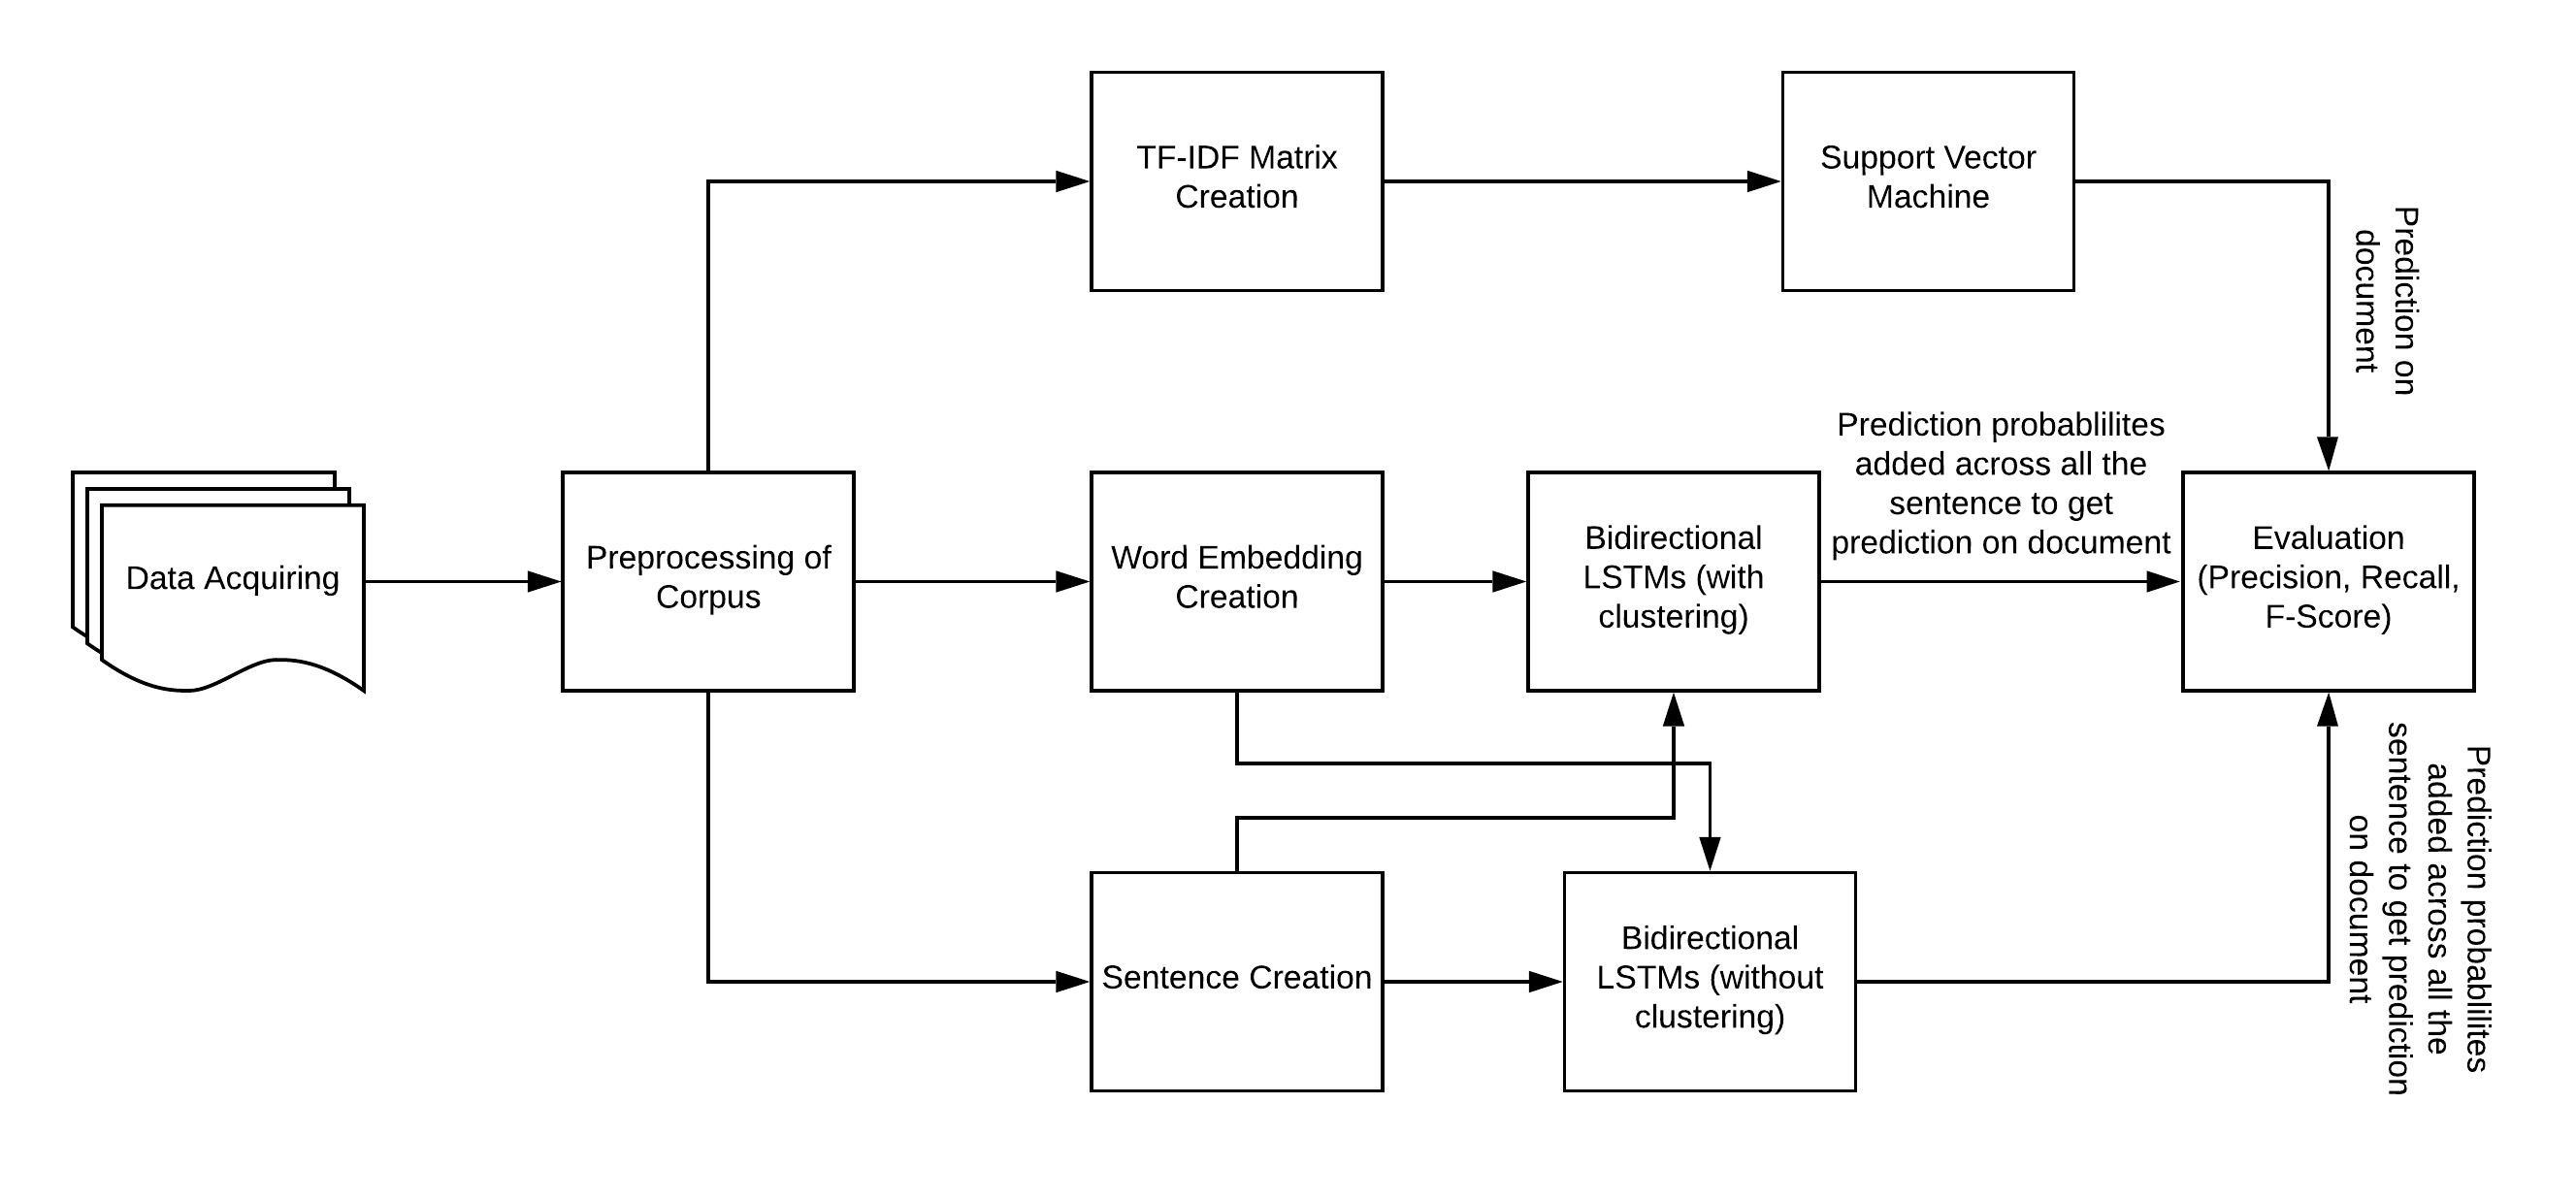
\includegraphics[width=15cm, height=14cm,keepaspectratio]{pics/flowforQuestion1.jpeg}
    \caption{Flow chart representing the workflow for the first research question }
    \label{fig:FlowResearchQuestion1}
\end{figure}

Two LSTM models are trained to see the effects of clustering. The training workflow for the Bidirectional LSTM (with clustering) is shown below in \ref{fig:clusterFlowClassification},

\begin{figure}[!ht]
    \centering
    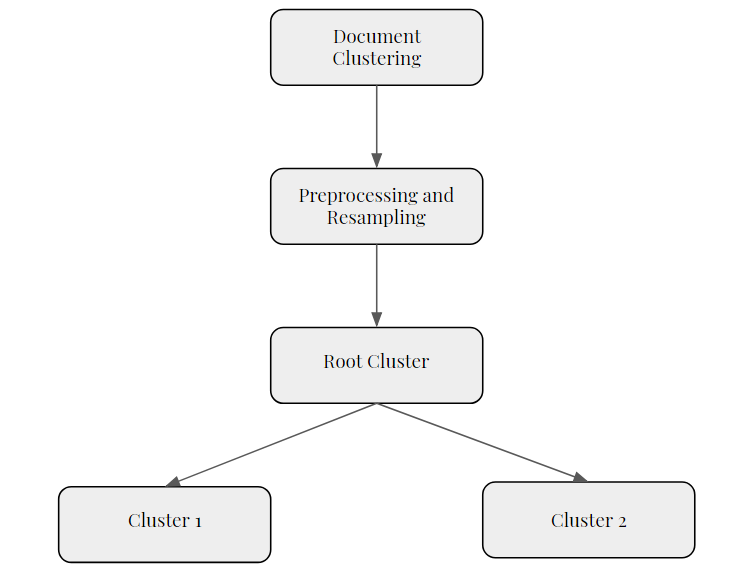
\includegraphics[width=10cm,keepaspectratio]{pics/clusterClassificationFlow.png}
    \caption{Classification workflow for clustered data}
    \label{fig:clusterFlowClassification}
\end{figure}

\subsubsection*{Evaluation} \label{evaluationQuestionOne}
As the SVMs are trained on full documents and LSTMs are trained on sentences created using sliding window technique, the results from both can not be compared. Ferguson et al.,(2009) preformed sentiment analysis of the financial blogs on paragraph-level 
annotated text, they summed up the predictions given by the classifier. In our case, the classifier will give probability to each sentence belonging to each class. As each document comprises of sentences, if we add all the probabilities for each class across all the sentences of a document we get probabilities of each class for that document and then we choose the class with highest probability.

\subsection{Research Question 2:} \label{question2}
The second research question is:

\begin{quote}
    Are general-purpose resources such as \textit{pre-trained word embeddings} in case of \textit{LSTM} applicable to specific legal domain tasks in terms of evaluation metrics? Also, further training them on legal corpus, produces comparable results to the ones only trained on legal texts?
\end{quote}

\begin{figure}[!ht]
    \centering
    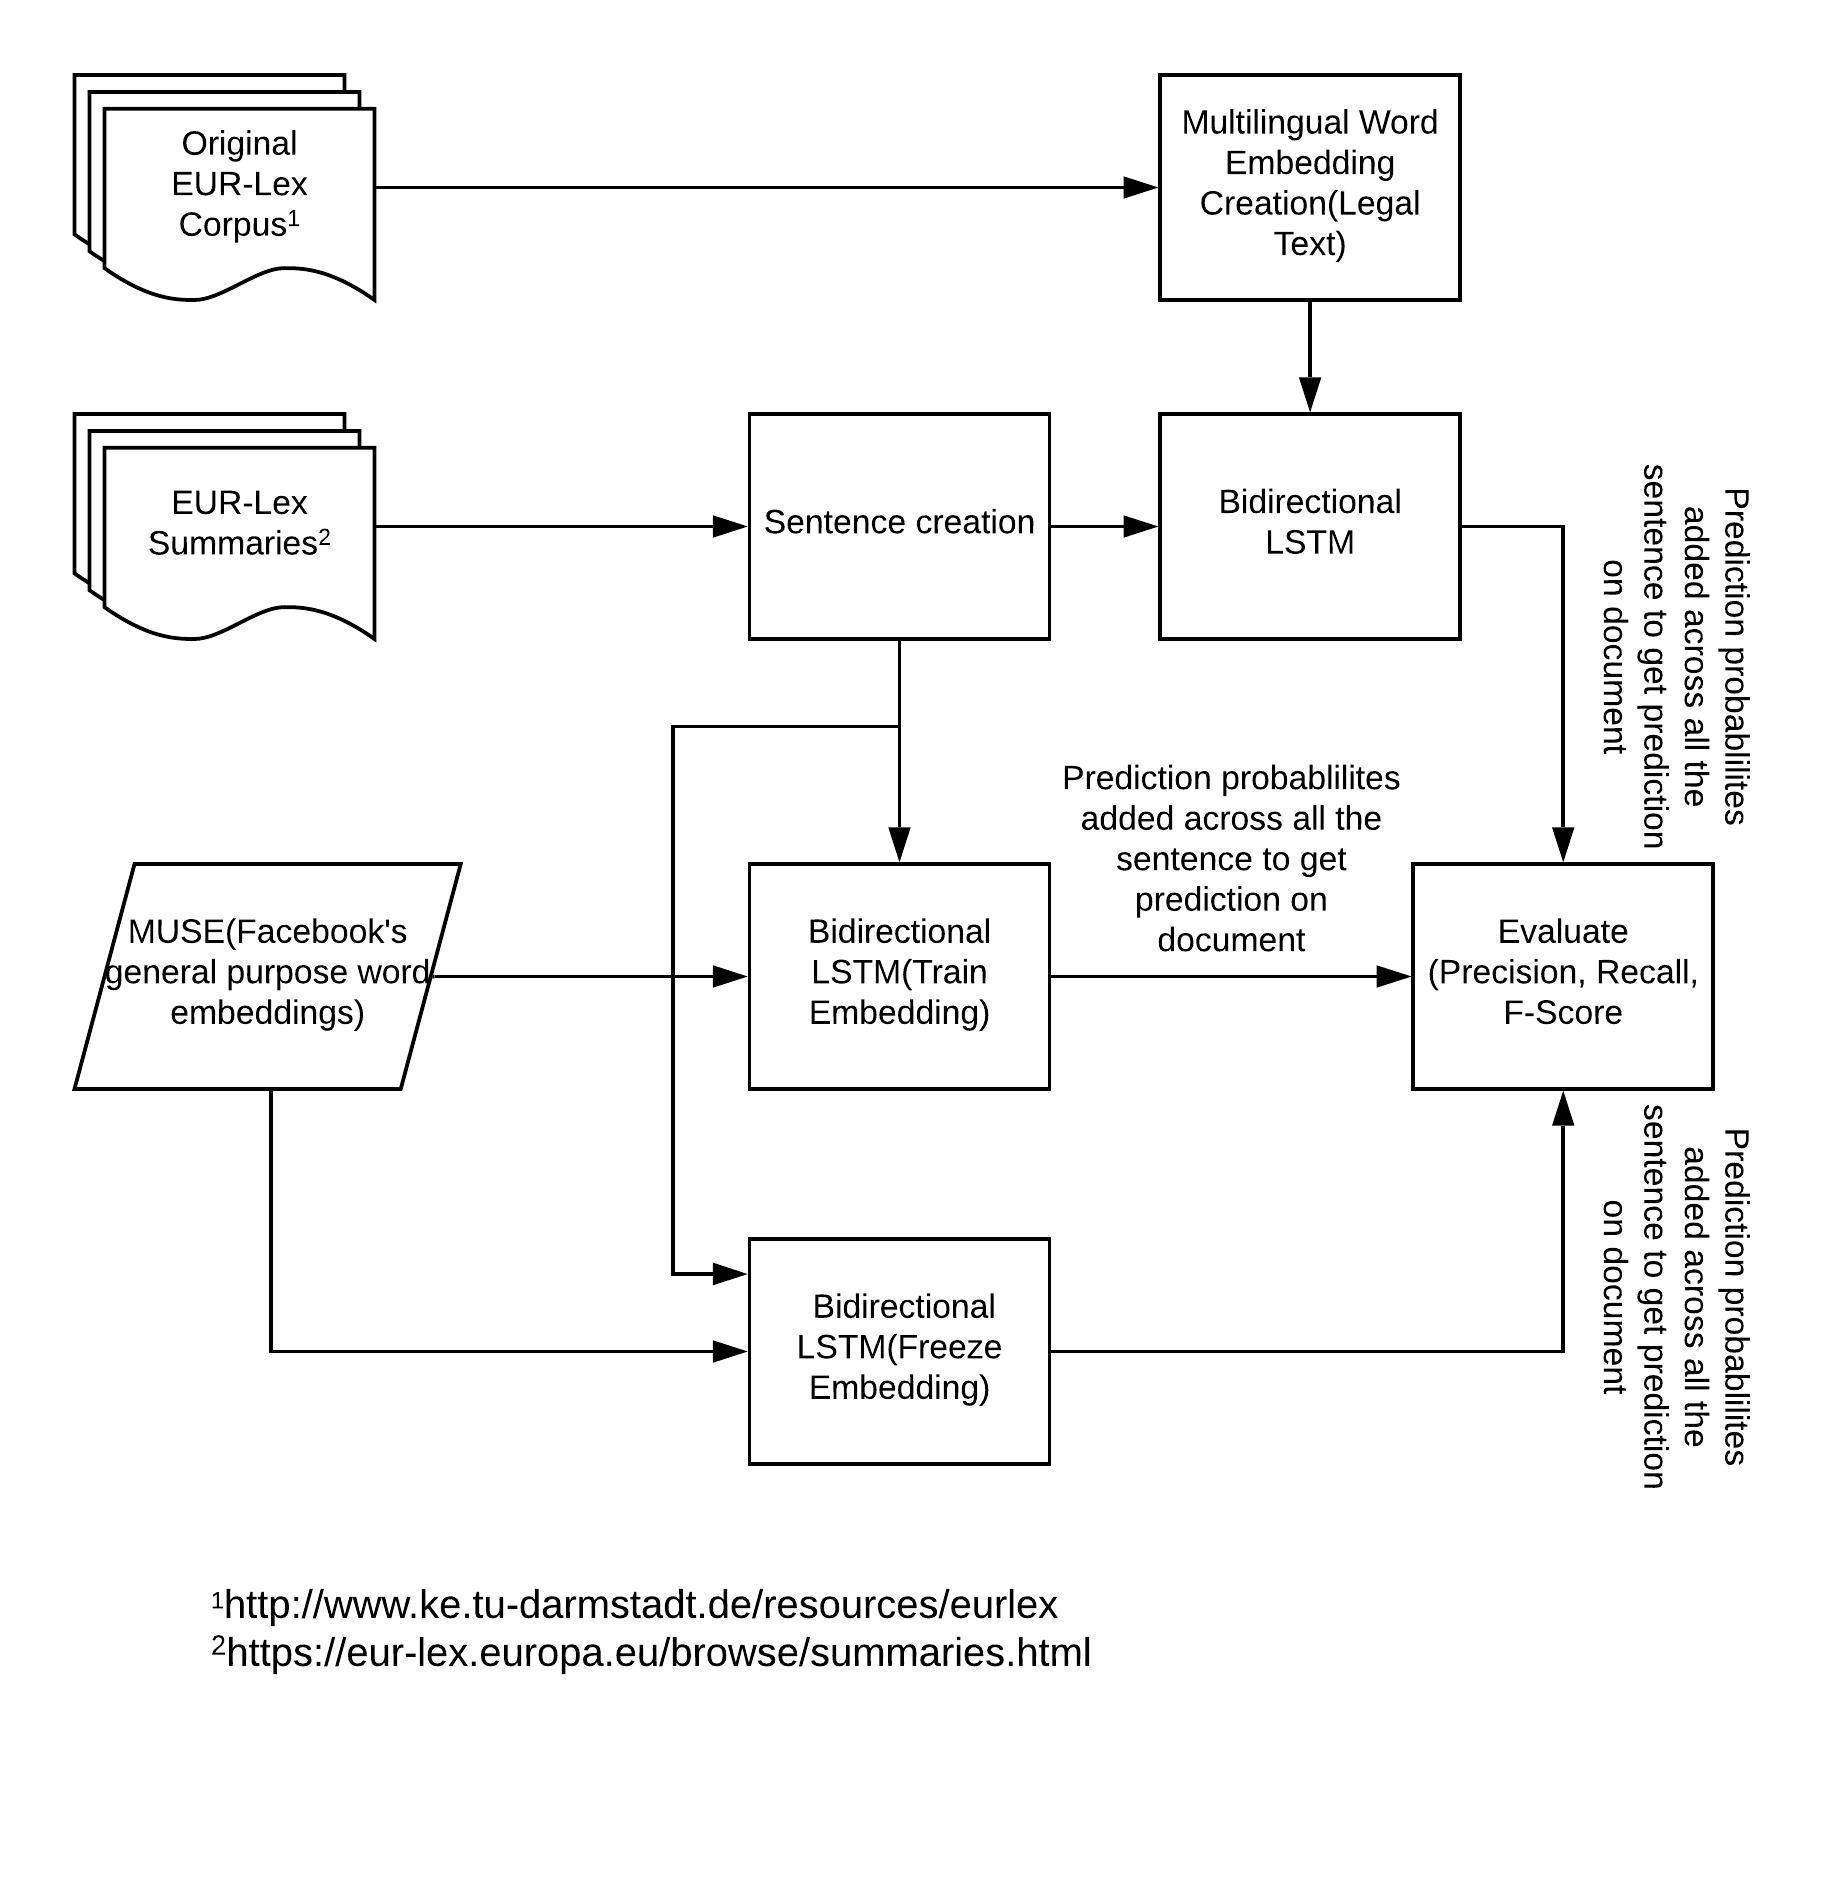
\includegraphics[width=15cm, height=14cm,keepaspectratio]{pics/flowforQuestion2.jpeg}
    \caption{Flow chart representing the workflow for the second research question}
    \label{fig:FlowResearchQuestion2}
\end{figure}

\ref{fig:FlowResearchQuestion2} shows the general workflow for the second question we compare the general purpose resources, that is word embeddings for training LSTM, with the word embeddings trained on legal corpus. Facebook's Fasttext\footnote{https://fasttext.cc/docs/en/crawl-vectors.html}\cite{graves2009novel} provides word vectors in 157 languages on Wikipedia\footnote{https://www.wikipedia.org/} and Common Crawl\footnote{http://commoncrawl.org/} data and is trained using Continuous bag-of-words model in dimension 300, with character n-grams of length 5, a window of size 5 and 10 negatives. But as the word embeddings for multiple languages can not be combined together because they belong in different vector space. Facebook's MUSE\footnote{https://github.com/facebookresearch/MUSE} \cite{conneau2017word} with help of parallel dictionaries was used to align them in a single vector space. After this both embeddings can be simply concatenated and can be used for classification purpose. 

For creating domain specific word embeddings Duong et al.(2016)\cite{duong-EtAl:2016:EMNLP} proposed learning bilingual word embedding without without bilingual Corpora\cite{duong-EtAl:2016:EMNLP}. They also make use of parallel bilingual dictonaries and use Continuous bag-of-word model to create these embeddings. These word embeddings are however in a single vector space.

As the domain specific word embeddings are create using legal domain specific data this word embedding will not be further trained. In case of general purpose word embeddings two models will be trained - one with frozen embedding layer and other model will train the word embeddings. This is done to see if training the general purpose word embeddings produces results comparable to the ones trained on legal data.

Similar to the first question all the models will be trained on clustered data as shown in \ref{fig:clusterFlowClassification} and the evaluation will also be done similar to question one (See \ref{evaluationQuestionOne}).

\subsection{Research Question 3:} \label{question3}

The third research question is:

\begin{quote}
    Can \textit{LSTM} perform better  when a single model is trained on multiple languages, compared to training one model for each language separately?
\end{quote}

\ref{fig:FlowResearchQuestion3} shows the general workflow for the third research question. In this question we explore the possible effects of having data in multiple languages on a classifier. C.-P. Wei et al.(2014)\cite{Wei:2014:EPD:2566999.2567111} suggested that when training set for a single language is small it is less representative target semantic space and a classifier trained on this data set would not yield satisfactory results. However, if text from another language is available for the predefined category then it can be beneficial to improve the effectiveness of the classifier for the previous language. The naïve approaches of handling such data is to build separate classifiers for separate languages. This naïve method does not take the benefit of availability of data across different language for a defined category. 

In this research question, first two separate classifiers will be trained on two different languages namely, \textit{English} and \textit{German}. The results from both of them will be combined to get the average performance (we will average the macro-average precision, recall, and f-score across both the models) of classification of these two classifiers. The training and evaluation of these classifiers will be similar to the training done in question 1 and 2. This performance of the two classifiers will then be compared to a single classifiers that will be trained on both the languages with multilingual word embeddings.

The training of all the classifiers for this question will be done in the similar fashion as show in \ref{fig:clusterFlowClassification}.


\begin{figure}[!ht]
    \centering
    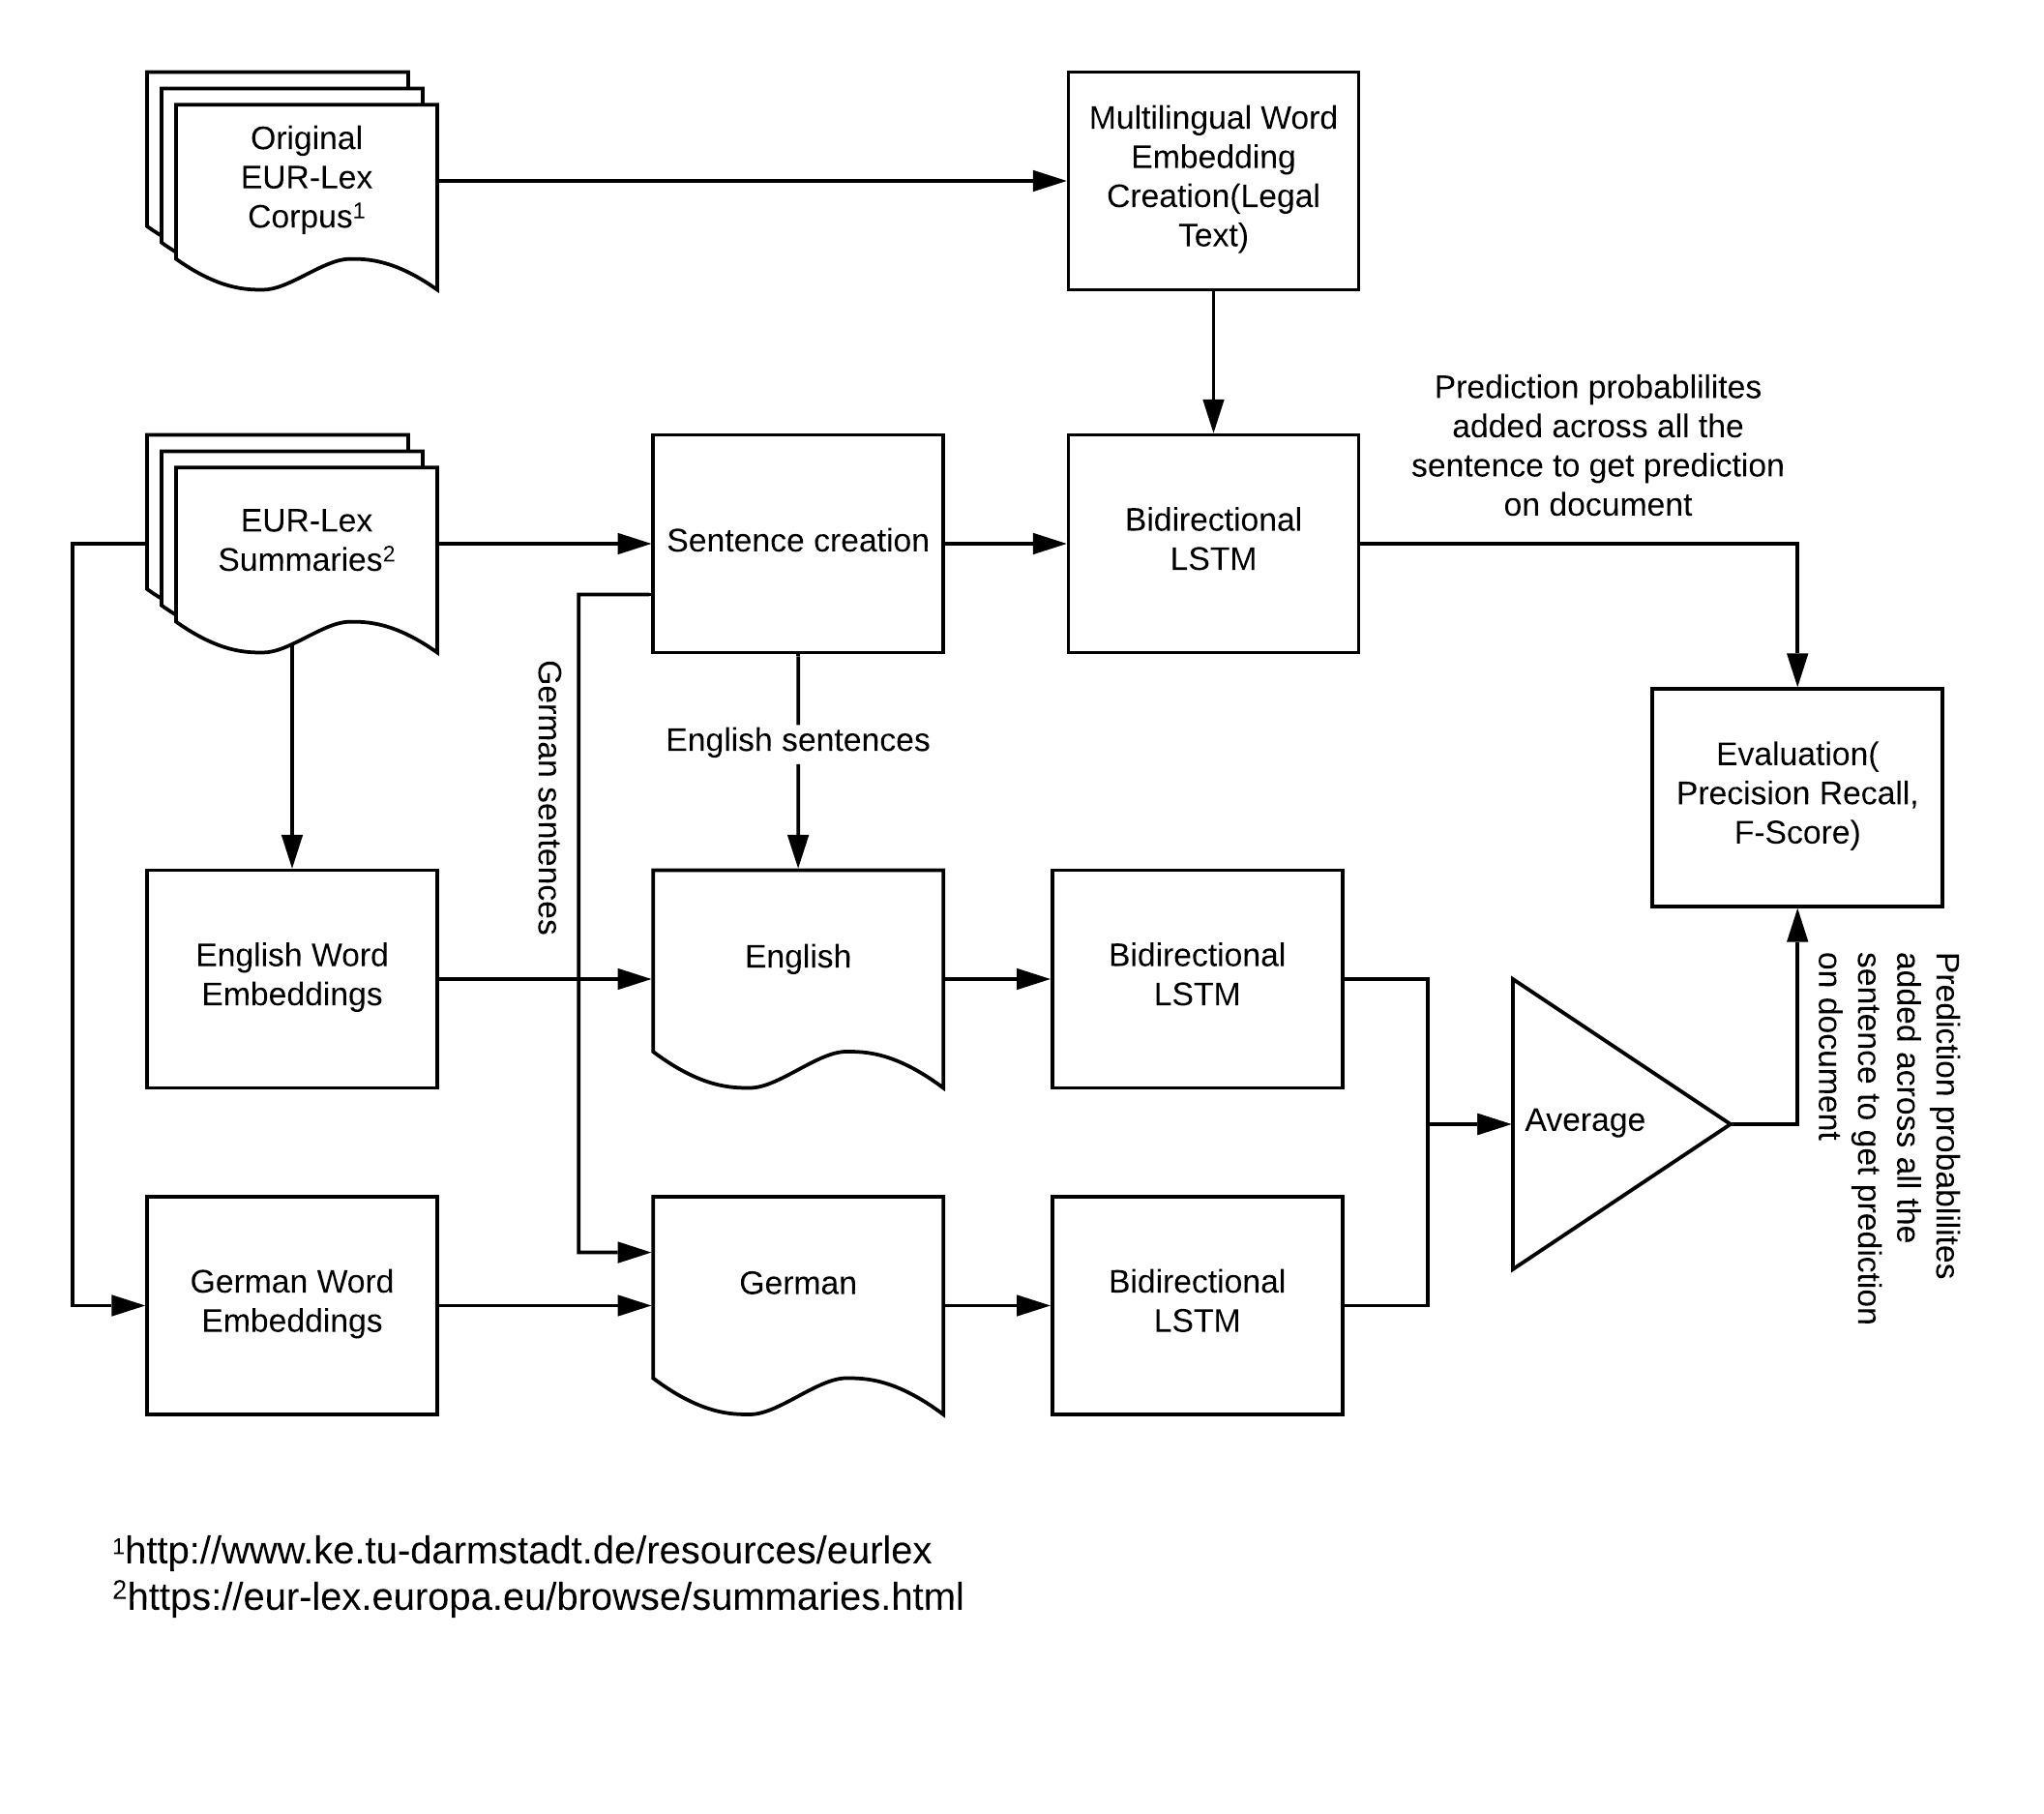
\includegraphics[width=15cm, height=14cm,keepaspectratio]{pics/flowforQuestion3.jpeg}
    \caption{Flow chart representing the workflow for the third research question}
    \label{fig:FlowResearchQuestion3}
\end{figure}